% IS-RAG — arXiv preprint, standalone (no ACL .sty required)
% Compiles with: pdflatex main.tex  (twice, then bibtex, twice again)
% Requires standard TeX Live packages only.
\documentclass[11pt,a4paper]{article}

% --- Layout ---
\usepackage[margin=2.5cm]{geometry}
\usepackage{multicol}           % two-column body (optional, comment out for single)
\usepackage{titlesec}
\usepackage{parskip}

% --- Fonts & Encoding ---
\usepackage[T1]{fontenc}
\usepackage[utf8]{inputenc}
\usepackage{times}
\usepackage{microtype}

% --- Math ---
\usepackage{amsmath,amssymb}

% --- Tables & Figures ---
\usepackage{booktabs}
\usepackage{graphicx}
\usepackage{multirow}
\usepackage{array}
\usepackage{caption}
\usepackage{float}

% --- Lists ---
\usepackage{enumitem}

% --- Color ---
\usepackage{xcolor}

% --- Algorithms ---
\usepackage{algorithm}
\usepackage{algpseudocode}
\renewcommand{\algorithmicrequire}{\textbf{Input:}}
\renewcommand{\algorithmicensure}{\textbf{Output:}}

% --- Code listings ---
\usepackage{listings}
\lstset{
  basicstyle=\ttfamily\small,
  breaklines=true,
  frame=single,
  backgroundcolor=\color{gray!8},
  columns=fullflexible,
  keepspaces=true,
  literate={á}{{\'a}}1 {ã}{{\~a}}1 {â}{{\^a}}1 {à}{{\`a}}1
           {é}{{\'e}}1 {ê}{{\^e}}1
           {í}{{\'i}}1
           {ó}{{\'o}}1 {ô}{{\^o}}1 {õ}{{\~o}}1
           {ú}{{\'u}}1 {ü}{{\"u}}1
           {ç}{{\c{c}}}1
           {Á}{{\'A}}1 {Ã}{{\~A}}1 {É}{{\'E}}1 {Ó}{{\'O}}1 {Ú}{{\'U}}1
}

% --- Hyperlinks ---
\usepackage[colorlinks=true,linkcolor=blue!70!black,citecolor=blue!70!black,urlcolor=blue!70!black]{hyperref}

% --- Bibliography ---
\usepackage[round,sort,authoryear]{natbib}
\bibliographystyle{plainnat}

% --- Section formatting (ACL-like) ---
\titleformat{\section}{\normalsize\bfseries}{\thesection.}{0.5em}{}
\titleformat{\subsection}{\normalsize\itshape}{\thesubsection.}{0.5em}{}
\titleformat{\paragraph}[runin]{\normalsize\bfseries}{}{0pt}{}[~~]
\titlespacing{\section}{0pt}{6pt}{3pt}
\titlespacing{\subsection}{0pt}{4pt}{2pt}

% --- Figure placeholder ---
\newcommand{\figplaceholder}[2]{%
  \begin{center}
    \fbox{\parbox[c][#1][c]{0.92\linewidth}{%
      \centering\color{gray}\small [Figure — #2]%
    }}
  \end{center}%
}

% --- Abstract environment ---
\renewenvironment{abstract}{%
  \small\begin{center}{\bfseries Abstract}\end{center}%
  \begin{quote}\small
}{%
  \end{quote}\bigskip
}

% =================================================================
\begin{document}

% --- Title block ---
\begin{center}
  {\Large\bfseries IS-RAG: Image-Schematic Retrieval-Augmented\\
   Generation for Cognitive Search in Political Discourse}

  \vspace{0.8em}

  {\normalsize
    Yan Justino$^{1,2}$ \\[4pt]
    $^1$ CESAR School \quad $^2$ Itaú Unibanco \\[4pt]
    \texttt{contact@yanjustino.com}
  }

  \vspace{0.6em}
  \rule{\linewidth}{0.4pt}
\end{center}

% =================================================================
\begin{abstract}
\textbf{Objective.}
Dense retrieval systems fail when the user and the document express
the same conceptual structure through distinct vocabularies — a
phenomenon we term the \emph{lexical-cognitive gap}.
This paper presents \textbf{IS-RAG}, a pilot study that investigates
whether explicit indexing of \emph{image schemas}
\citep{lakoff1980,talmy1988} — pre-linguistic patterns such as
\textsc{Force}, \textsc{Container}, and \textsc{Path} — can bridge
this gap in a corpus of Portuguese political discourse.

\textbf{Method.}
During indexing, an LLM-based \emph{Cognitive Parser} annotates each
chunk with the image schemas present, generating structured metadata
stored alongside two independent vector embeddings: one textual and
one cognitive.
At query time, schemas detected in the query trigger a
\emph{proportional boost} over chunks sharing the same cognitive
structure, enabling retrieval driven by abstract spatial metaphor
beyond lexical overlap.

\textbf{Evaluation.}
We construct a TREC-style ground truth over 121 Brazilian
parliamentary speeches (171 chunks), with 10 valid queries
(3~\textsc{Force} $+$ 3~\textsc{Container} $+$ 3~\textsc{Path} $+$
1~cross-schema) annotated by an independent LLM
(\texttt{claude-opus-4-7}, distinct from the Cognitive Parser) on a
0--3 scale.
The primary metric is NDCG@5; the baseline is dense retrieval without
cognitive boosting.

\textbf{Findings.}
An ablation over three retrieval modes reveals that
\emph{text-mode boosting} — proportional cognitive boosting applied
over text-embedding similarity — is the most effective configuration,
achieving a mean NDCG@5 of 0.7793 vs.\ 0.6881 for the baseline
($\Delta = +0.091$).
Using the cognitive embedding as the primary search vector degrades
performance ($\Delta_\text{cognitive} = -0.192$;
$\Delta_\text{hybrid} = -0.090$), localising the IS-RAG contribution
in the boosting mechanism rather than in dual-embedding retrieval.
\textsc{Force} queries benefit most consistently
($\Delta_\text{FORCE} = +0.267$); \textsc{Path} is net positive
across all three queries ($\Delta_\text{PATH} = +0.085$);
\textsc{Container} shows a near-zero mean effect
($\Delta_\text{CONT} = -0.017$).
Two additional methodological findings emerge: (1)~queries must be
formulated as \emph{assertive metaphorical statements} to activate
the cognitive component; (2)~schema frequency in the corpus does not
predict \emph{boostability} — conventionalised schemas carry no
discriminative re-ranking signal.
\end{abstract}

\noindent\textbf{Keywords:} retrieval-augmented generation $\cdot$ image schemas $\cdot$ cognitive linguistics $\cdot$ information retrieval $\cdot$ natural language processing $\cdot$ metaphor detection $\cdot$ dense retrieval $\cdot$ political discourse $\cdot$ semantic search $\cdot$ embodied cognition

% =================================================================
\section{Introduction}
\label{sec:intro}

Retrieval-Augmented Generation \citep{lewis2020rag} typically grounds
document retrieval in surface-level lexical or dense semantic
similarity.
This works well when query vocabulary overlaps with document
vocabulary, but breaks down under a \emph{lexical-cognitive gap}: the
user and the document express the same conceptual structure using
different words, often because both rely on underlying bodily
metaphors that map physical spatial experience onto abstract domains
\citep{johnson1987,lakoff1980}.

Consider a query about \emph{economic pressure on households} and a
parliamentary speech about \emph{institutions blocking each other in a
constitutional dispute}. Both invoke the image schema
\textsc{Force}/\textsc{Compulsion}—an external agent exerting force on
a patient—yet their vocabularies share little overlap, making standard
dense retrieval unable to bridge the gap.

\emph{Image schemas} \citep{johnson1987,feldman2006} are
pre-linguistic, embodied patterns (\textsc{Container}, \textsc{Path},
\textsc{Force}) that recur as structural metaphors across every domain
of abstract reasoning.
We hypothesise that indexing these schemas explicitly and matching them
at query time enables a form of deep structural retrieval that
complements dense semantic search.

\paragraph{Contributions.}
\begin{itemize}[noitemsep,topsep=2pt]
  \item We present IS-RAG, a technique that indexes image-schema
        metadata alongside dual vector embeddings (text and cognitive)
        and applies proportional cognitive boosting at retrieval time
        (\S\ref{sec:method}).
  \item We construct a TREC-style ground truth over a real corpus of
        Brazilian parliamentary speeches (171 chunks, 9 valid queries,
        LLM-as-annotator) and report NDCG@5 (\S\ref{sec:eval}).
  \item We identify methodological constraints for schema-aware
        retrieval evaluation: assertive query formulation, schema
        frequency vs.\ annotability, and LLM circularity risk
        (\S\ref{sec:discussion}).
\end{itemize}

% =================================================================
\section{Related Work}
\label{sec:related}

\paragraph{Retrieval-Augmented Generation.}
\citet{lewis2020rag} introduced RAG to ground generation in retrieved
passages. Dense retrieval over bi-encoder representations
\citep{karpukhin2020dpr} has become the standard backbone. Extensions
explore hybrid sparse-dense search, re-ranking, and structured
knowledge augmentation, but none incorporate pre-linguistic spatial
metaphor as a retrieval signal.

\paragraph{Metaphor in NLP.}
Automatic metaphor detection has been studied as classification or
span extraction \citep{shutova2010,tsvetkov2014}.
\citet{wachowiak2023,wachowiak-gromann-2022-systematic} explore LLMs for metaphor identification. These
works focus on metaphor \emph{detection}; IS-RAG is the first, to our
knowledge, to use detected image-schema structure as a
\emph{retrieval scoring signal}.

\paragraph{Cognitive Linguistics and IR.}
Image schemas as cognitive universals were formalised by
\citet{lakoff1980}, \citet{johnson1987}, and \citet{talmy1988}.
\citet{feldman2006} discusses their neural basis. No prior IR work
indexes documents by image schema and uses schema matching for
retrieval boosting.

\paragraph{Portuguese NLP and parliamentary corpora.}
Pre-trained language models for Brazilian Portuguese
\citep{souza2020bertimbau} have demonstrated that language-specific
pretraining substantially improves downstream performance relative to
generic multilingual models.
Parliamentary discourse in Portuguese has been studied through the
Corpus Ulysses \citep{albuquerque2022ulyssesner}, a collection of legislative
documents from the Brazilian Chamber of Deputies used for text
classification, named entity recognition, and semantic analysis.
Our evaluation corpus is drawn from the same institutional source
via the same open API and extends existing resources with
image-schema annotations and graduated relevance judgements for
retrieval evaluation.
Framing and sentiment analysis of Brazilian political text
\citep{vargas2021bert} provide further precedent for
computational approaches to ideological structure in Portuguese
parliamentary language.

% =================================================================
\section{Method}
\label{sec:method}

Figure~\ref{fig:pipeline} illustrates the IS-RAG pipeline. Formal
pseudo-code is given in Appendix~\ref{app:algorithms}.

\begin{figure}[h]
  \centering
  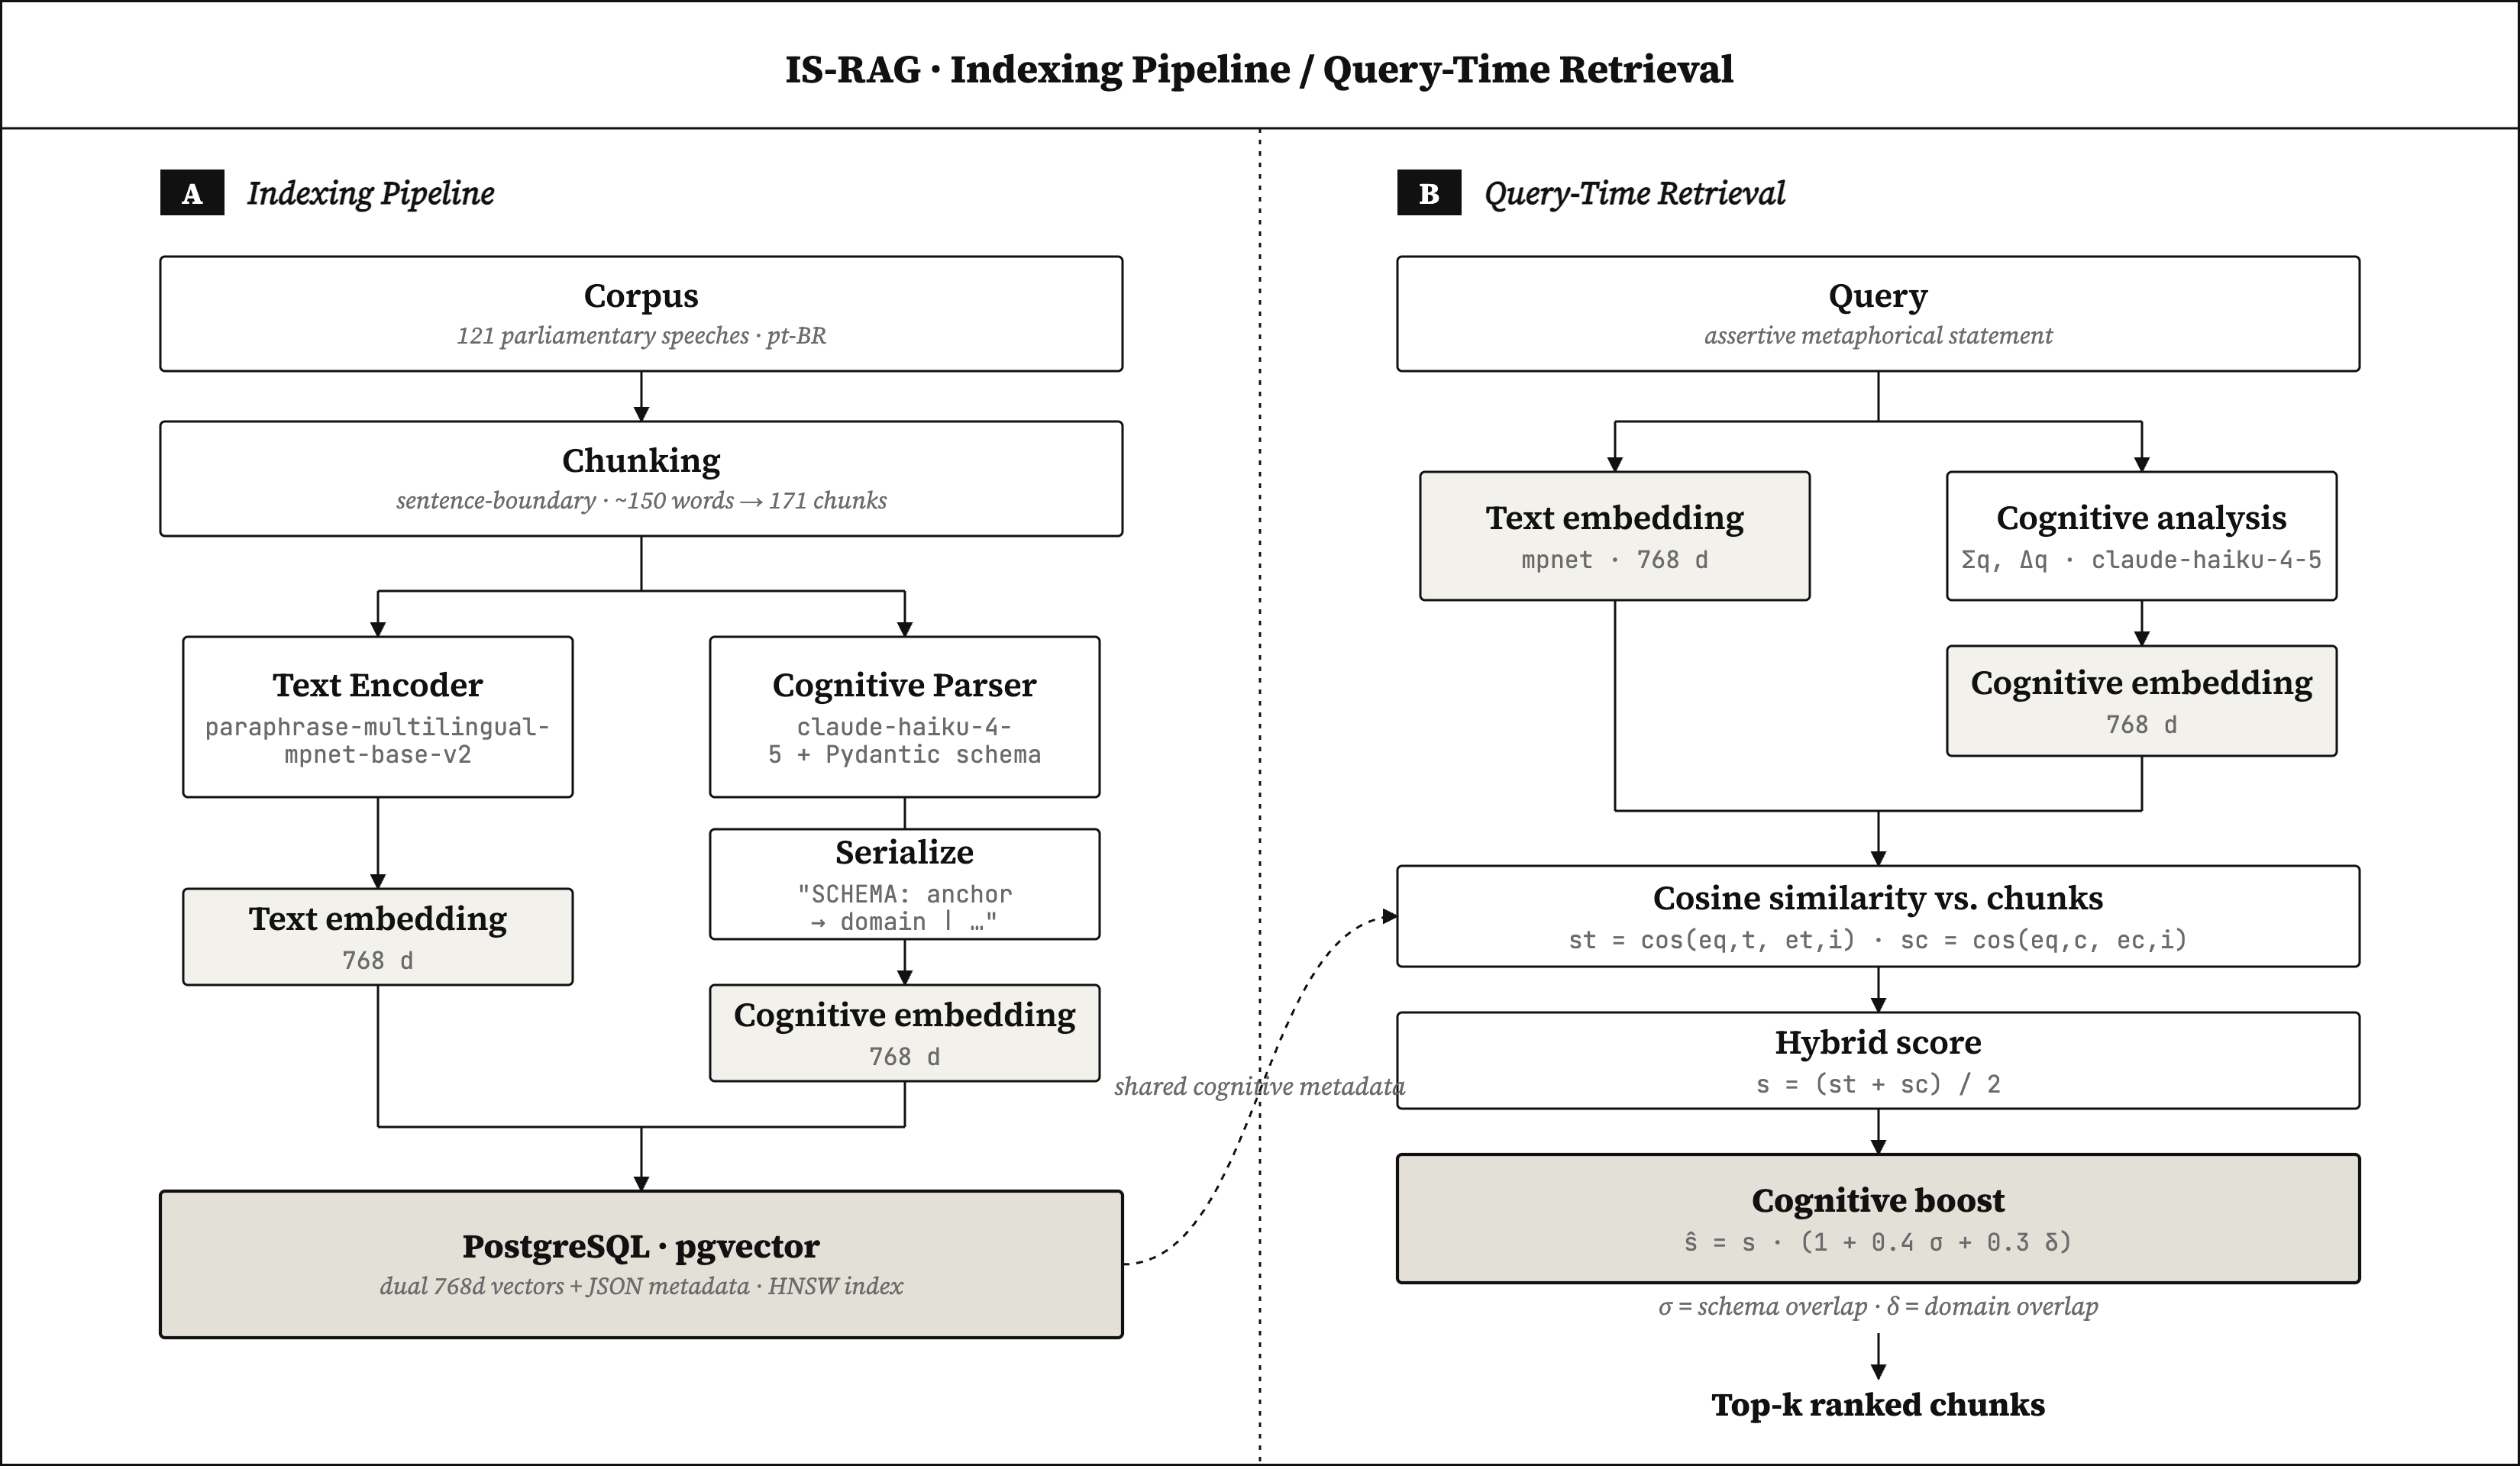
\includegraphics[width=1\textwidth]{images/EN_Pipeline_en-us_.png}
  \caption{IS-RAG overview: indexing and retrieval steps.}
  \label{fig:pipeline}
\end{figure}

\subsection{Corpus and Chunking}

The corpus comprises 121 Brazilian parliamentary speeches in
\textbf{Portuguese}, collected from the open API of the Brazilian
Chamber of Deputies (\url{dados.camara.leg.br/api/v2}), spanning
January–December~2025.
Speeches are stratified by ideological spectrum (left, centre, right)
across 13 parties.
Each speech is segmented into chunks of approximately 150~words using
sentence-boundary splitting, yielding 171~chunks (mean 2.7 per
speech).

\subsection{Dual Embeddings}

Each chunk produces two independent 768-dimensional vectors:

\begin{enumerate}[noitemsep,topsep=2pt]
  \item \textbf{Text embedding:} dense representation of the raw chunk
        text via \textit{paraphrase-multilingual-mpnet-base-v2}
        \citep{reimers2019sbert}, running locally on CPU.
  \item \textbf{Cognitive embedding:} dense representation of the
        serialised cognitive metadata in the form
        \texttt{"SCHEMA: anchor $\to$ domain $|$ \ldots"}, capturing
        image-schematic structure independently of literal vocabulary.
\end{enumerate}

Both vectors are stored in PostgreSQL~16 with the \texttt{pgvector}
extension and indexed via HNSW for approximate nearest-neighbour
search.

We deliberately chose \texttt{paraphrase-multilingual-mpnet-base-v2}
over more recent commercial embedding APIs for two reasons.
First, \emph{reproducibility}: all embeddings are generated locally
without API access, rate limits, or usage costs, enabling full
replication of the experiment.
Second, \emph{adequacy}: the model provides validated coverage of
Portuguese within a 768-dimensional space sufficient for the
proof-of-concept scale of this work (171~chunks), and its
multilingual training includes Brazilian Portuguese
\citep{souza2020bertimbau}.
We do not claim that upgrading to larger or more recent embedding
models would not improve results; this is an explicit agenda item
(\S\ref{sec:conclusion}) but is orthogonal to the variable under
investigation—the cognitive boosting signal itself.

\subsection{Cognitive Parser}

The Cognitive Parser sends each chunk to
\texttt{claude-haiku-4-5} \citep{anthropic2024} using a shared prompt
(available at \url{https://github.com/yanjustino/is-rag}) and extracts structured JSON validated by
a Pydantic schema. The taxonomy follows \citet{lakoff1980} and
\citet{talmy1988}:

\begin{center}
\small
\begin{tabular}{ll}
\toprule
\textbf{Schema} & \textbf{Subtypes} \\
\midrule
\textsc{Container} & Inside, Outside, Boundary, Intrusion \\
\textsc{Path}      & Source, Trajectory, Goal, Diversion \\
\textsc{Force}     & Blockage, Compulsion, Resistance, Counter\_Force \\
\bottomrule
\end{tabular}
\end{center}

A \emph{literality rule} instructs the model to return empty lists for
non-metaphorical text, preventing hallucinated schemas.
Chunks are processed concurrently (5 workers) to reduce ingestion
time.
The corpus yields 92~\textsc{Path}, 88~\textsc{Container}, and
83~\textsc{Force} schema occurrences across the 171~chunks.

\subsection{Hybrid Search and Cognitive Boosting}
\label{sec:boosting}

IS-RAG supports three retrieval modes.
In all three, the Cognitive Parser runs on the query at retrieval time
to detect schemas ($\Sigma_q$) and target domains ($\Delta_q$).
The modes differ only in how the base similarity~$s$ is computed
before the boost:

\begin{itemize}[noitemsep,topsep=2pt]
  \item \textbf{Text:} $s = \cos(\mathbf{e}_{q,t},\,\mathbf{e}_{t,i})$
        — the query's raw-text embedding is matched against chunk text
        embeddings.  The cognitive information contributes only via the
        boost.
  \item \textbf{Cognitive:} $s = \cos(\mathbf{e}_{q,c},\,\mathbf{e}_{c,i})$
        — the query's Cognitive Parser output is serialised using the
        same \texttt{schema\,$\to$\,domain} format as indexing,
        embedded, and matched against chunk cognitive embeddings.
  \item \textbf{Hybrid:} $s = \bigl(s_t + s_c\bigr)/2$
        — arithmetic mean of text and cognitive similarities.
\end{itemize}

After computing~$s$, the same \emph{proportional cognitive boost} is
applied in all three modes:

\begin{equation}
  \label{eq:boosting}
  \hat{s} = s \cdot \bigl(1 + 0.4\,\sigma + 0.3\,\delta\bigr)
\end{equation}

\noindent where $\sigma$ is the fraction of a chunk's cognitive
details whose \texttt{schema\_name} matches a schema in~$\Sigma_q$,
and $\delta$ is the analogous fraction for \texttt{target\_domain}
against~$\Delta_q$.
Weights ($\alpha{=}0.4$, $\beta{=}0.3$) were set by design; schema
structure is the primary signal, domain the secondary reinforcement.
The baseline disables the Cognitive Parser entirely and applies pure
text-embedding retrieval without boosting.

% =================================================================
\section{Evaluation Setup}
\label{sec:eval}

\paragraph{Ground Truth Construction.}
We construct a TREC-style pooled ground truth
\citep{voorhees2005}.
For each query, IS-RAG (hybrid) and the baseline independently
retrieve the top-10 chunks; the union ($\approx$14--18 unique chunks
per query) is annotated for relevance~(0--3) by an LLM
(\texttt{claude-opus-4-7}).
Scores~$\geq 2$ require the annotator to cite an anchor word and
schema subtype as traceable evidence.
Queries with IDCG$=0$ (no chunk with score~$\geq 2$) are excluded
\citep{buckley2004}; this criterion triggered the exclusion of one
query (see \S\ref{sec:discussion}).

\paragraph{Query Design.}
Ten valid queries are designed with three properties:
(1)~taxonomic coverage (3~\textsc{Force} $+$ 3~\textsc{Container} $+$
3~\textsc{Path} $+$ 1~cross-schema);
(2)~deliberate lexical gap (queries use assertive metaphorical
language, avoiding the literal vocabulary expected in documents);
(3)~cross-domain scenarios (queries target schemas that appear in
domains other than the query's own domain).

\paragraph{Metric.}
We report NDCG@5 \citep{jarvelin2002}.
MRR was rejected: with multiple relevant documents at different
relevance grades, MRR saturates at~1.0 regardless of ranking quality
\citep{buckley2004}.

% =================================================================
\section{Results}
\label{sec:results}

\subsection{Retrieval Mode Ablation}
\label{sec:ablation}

Table~\ref{tab:modes} compares all three IS-RAG retrieval modes against
the baseline.
Text mode is the only configuration that surpasses the baseline;
cognitive and hybrid modes both degrade retrieval.

\begin{table}[h]
\centering
\small
\setlength{\tabcolsep}{6pt}
\begin{tabular}{lccc}
\toprule
\textbf{Mode} & \textbf{IS-RAG} & \textbf{Baseline} & $\boldsymbol{\Delta}$ \\
\midrule
\textbf{Text}  & \textbf{0.7793} & 0.6881 & \textbf{+0.091} \\
Hybrid         & 0.5979          & 0.6881 & $-$0.090 \\
Cognitive      & 0.4958          & 0.6881 & $-$0.192 \\
\midrule
Baseline       & —               & 0.6881 & — \\
\bottomrule
\end{tabular}
\caption{Mean NDCG@5 across 10 queries by retrieval mode
  (independent Opus annotator).
  Text mode is the strongest IS-RAG configuration.}
\label{tab:modes}
\end{table}

Table~\ref{tab:modes_compare} breaks down $\Delta$ NDCG@5 per query
across all three modes, revealing which queries and schema families
drive the aggregate results.

\begin{table}[h]
\centering
\small
\setlength{\tabcolsep}{4pt}
\begin{tabular}{clccc}
\toprule
\textbf{Q} & \textbf{Schema / Domain} & \textbf{$\Delta$ Text} & \textbf{$\Delta$ Cog.} & \textbf{$\Delta$ Hyb.} \\
\midrule
Q1  & \textsc{Cont.}/Inside / Health            & 0.000           & $-$0.396        & $-$0.362 \\
Q2  & \textsc{Force}/Compulsion / Economics    & \textbf{+0.390} & +0.138          & +0.138 \\
Q3  & \textsc{Force}/Counter\_F / Justice      & \textbf{+0.221} & $-$0.504        & $-$0.277 \\
Q4  & \textsc{Force}/Resistance / Politics     & \textbf{+0.189} & +0.236          & +0.150 \\
\midrule
Q5  & \textsc{Cont.}/Intrusion / Justice       & $-$0.096        & $-$0.221        & $-$0.191 \\
Q6  & \textsc{Cont.}/Outside / Human Rights    & +0.046          & $-$0.172        & +0.046 \\
\midrule
Q7  & \textsc{Path}/Trajectory / Economics     & +0.036          & $-$0.188        & $-$0.007 \\
Q8  & \textsc{Path}/Source / Politics          & \textbf{+0.111} & $-$0.555        & $-$0.424 \\
Q9  & \textsc{Path}/Diversion / Politics       & +0.109          & $-$0.225        & +0.120 \\
\midrule
Q10 & \textsc{Force+Path} / Intl.\ Rel.        & $-$0.094        & $-$0.038        & $-$0.094 \\
\midrule
\multicolumn{2}{l}{\textbf{Mean}} & \textbf{+0.091} & $-$0.192 & $-$0.090 \\
\bottomrule
\end{tabular}
\caption{$\Delta$ NDCG@5 per query across all three IS-RAG modes
  (independent Opus annotator, 10~queries).
  Q1 (\textsc{Container}/\textsc{Inside}) shows $\Delta{=}0$ in text
  mode: the boost adds nothing for the most conventionalised subtype.
  Text mode is the most consistently positive across all families.}
\label{tab:modes_compare}
\end{table}

\paragraph{Why cognitive mode fails.}
In cognitive mode, serialised schema strings are the sole search
vectors.
With 171~chunks sharing overlapping schemas (PATH~92$\times$,
CONTAINER~88$\times$, FORCE~83$\times$), cosine similarities in this
space are tightly clustered, producing a noisy base ranking that
boosting cannot correct ($\Delta = -0.192$; Q8 degrades to
NDCG$\,{=}\,0.127$, Q1 to $0.127$).

\paragraph{Why hybrid mode fails.}
Hybrid mode averages $s_t$ and $s_c$ before boosting.
The noisy cognitive-embedding component contaminates the text signal,
pushing the base ranking below what pure text retrieval achieves
($\Delta = -0.090$).

\paragraph{Architectural implication.}
IS-RAG's value is a \emph{proportional re-ranking signal} derived from
schema metadata ($\sigma$,~$\delta$), not dual-embedding retrieval.
The \texttt{cognitive\_embedding} column is necessary for indexing
(computing $\sigma$) but counterproductive as a search vector.
Retaining \texttt{cognitive\_metadata} while using text-only similarity
as the base captures the full IS-RAG gain without the degradation
caused by hybrid or cognitive search.

\subsection{Robustness Validation: LLM Echo Effect}
\label{sec:robustness}

To rule out LLM echo as the source of the text-mode gain, we
re-annotated the relevance pool with \texttt{claude-opus-4-7}, a model
independent of the \texttt{claude-haiku-4-5} Cognitive Parser used at
indexing time.
Table~\ref{tab:annotator} reports text-mode NDCG@5 under both
annotators.
The $\Delta$ stays within one percentage point ($+0.091$ vs.\
$+0.093$); the independent annotator also resolves a previously
unannotable query (Q1 \textsc{Container}/\textsc{Inside}, IDCG${=}0$
with Haiku), expanding the evaluation to 10~valid queries.

\begin{table}[H]
\centering
\small
\setlength{\tabcolsep}{5pt}
\begin{tabular}{llcccc}
\toprule
\textbf{Annotator} & \textbf{Relation to parser} & \textbf{Queries} & \textbf{Baseline} & \textbf{IS-RAG} & \textbf{$\Delta$} \\
\midrule
\texttt{claude-haiku-4-5} & Same model & 9  & 0.6947 & 0.7873 & \textbf{+0.093} \\
\texttt{claude-opus-4-7}  & Independent & 10 & 0.6881 & 0.7793 & \textbf{+0.091} \\
\bottomrule
\end{tabular}
\caption{Text-mode NDCG@5 under two annotator configurations.
  The gain persists ($\Delta \approx +0.09$) under independent
  evaluation, ruling out LLM echo as the primary explanation.}
\label{tab:annotator}
\end{table}

\subsection{Embedding Utility Frontier}
\label{sec:embedding}

To test whether the text-mode gain survives a stronger base embedding,
we re-indexed the corpus with \texttt{BAAI/bge-m3} (1024d) and
re-annotated the pool with the same independent Opus annotator.
Table~\ref{tab:embedding} compares IS-RAG $\Delta$ across all three
modes for both models.
The text-mode gain collapses to $\Delta \approx 0$; hybrid and cognitive
degradation remain stable across models.
Q4 (\textsc{Force}/\textsc{Resistance}) drives the collapse: its
baseline rises from $0.489$ (mpnet) to $0.830$ (bge-m3), indicating the
stronger model already retrieves the correct documents without schema
assistance.

\begin{table}[H]
\centering
\small
\setlength{\tabcolsep}{4pt}
\begin{tabular}{lccc}
\toprule
\textbf{Embedding} & \textbf{$\Delta$ Text} & \textbf{$\Delta$ Hybrid} & \textbf{$\Delta$ Cognitive} \\
\midrule
\texttt{mpnet-base-v2} (768d) & \textbf{+0.091} & $-$0.090 & $-$0.192 \\
\texttt{bge-m3}        (1024d) & $\approx$0.001  & $-$0.068 & $-$0.202 \\
\bottomrule
\end{tabular}
\caption{IS-RAG $\Delta$ NDCG@5 across retrieval modes under two base
  embedding models (10~queries, independent Opus annotator).
  The text-mode gain is embedding-dependent: \texttt{bge-m3} closes the
  lexical-cognitive gap that IS-RAG compensated for with
  \texttt{mpnet-base-v2}.}
\label{tab:embedding}
\end{table}

\subsection{Per-Query Results (Text Mode)}

Table~\ref{tab:perquery} reports NDCG@5 for IS-RAG text mode —
the strongest configuration (\S\ref{sec:ablation}) — against the
baseline across all 10~valid queries (independent Opus annotator).

\begin{table}[h]
\centering
\small
\setlength{\tabcolsep}{4pt}
\begin{tabular}{clccc}
\toprule
\textbf{Q} & \textbf{Schema / Domain} & \textbf{IS-RAG} & \textbf{Base} & $\boldsymbol{\Delta}$ \\
\midrule
Q1  & \textsc{Cont.}/Inside / Health           & 0.5221 & 0.5221 & 0.000 \\
Q2  & \textsc{Force}/Compulsion / Economics    & 1.0000 & 0.6100 & \textbf{+0.390} \\
Q3  & \textsc{Force}/Counter\_F / Justice      & 0.9323 & 0.7116 & \textbf{+0.221} \\
Q4  & \textsc{Force}/Resistance / Politics     & 0.6787 & 0.4896 & \textbf{+0.189} \\
\midrule
Q5  & \textsc{Cont.}/Intrusion / Justice       & 0.7791 & 0.8754 & $-$0.096 \\
Q6  & \textsc{Cont.}/Outside / Human Rights    & 0.6993 & 0.6534 & +0.046 \\
\midrule
Q7  & \textsc{Path}/Trajectory / Economics     & 0.8200 & 0.7840 & +0.036 \\
Q8  & \textsc{Path}/Source / Politics          & 0.7929 & 0.6819 & \textbf{+0.111} \\
Q9  & \textsc{Path}/Diversion / Politics       & 0.7467 & 0.6377 & +0.109 \\
\midrule
Q10 & \textsc{Force+Path} / Intl.\ Rel.        & 0.8215 & 0.9155 & $-$0.094 \\
\midrule
\multicolumn{2}{l}{\textbf{Mean (10 queries)}} & \textbf{0.7793} & \textbf{0.6881} & \textbf{+0.091} \\
\bottomrule
\end{tabular}
\caption{NDCG@5 (IS-RAG text mode vs.\ baseline, independent Opus annotator).
  Queries grouped by schema family. All 10~valid queries shown.
  Q1 $\Delta{=}0$: cognitive boost is inert for conventionalised
  \textsc{Container}/\textsc{Inside}.}
\label{tab:perquery}
\end{table}

%\begin{figure}[h]
%  \centering
%  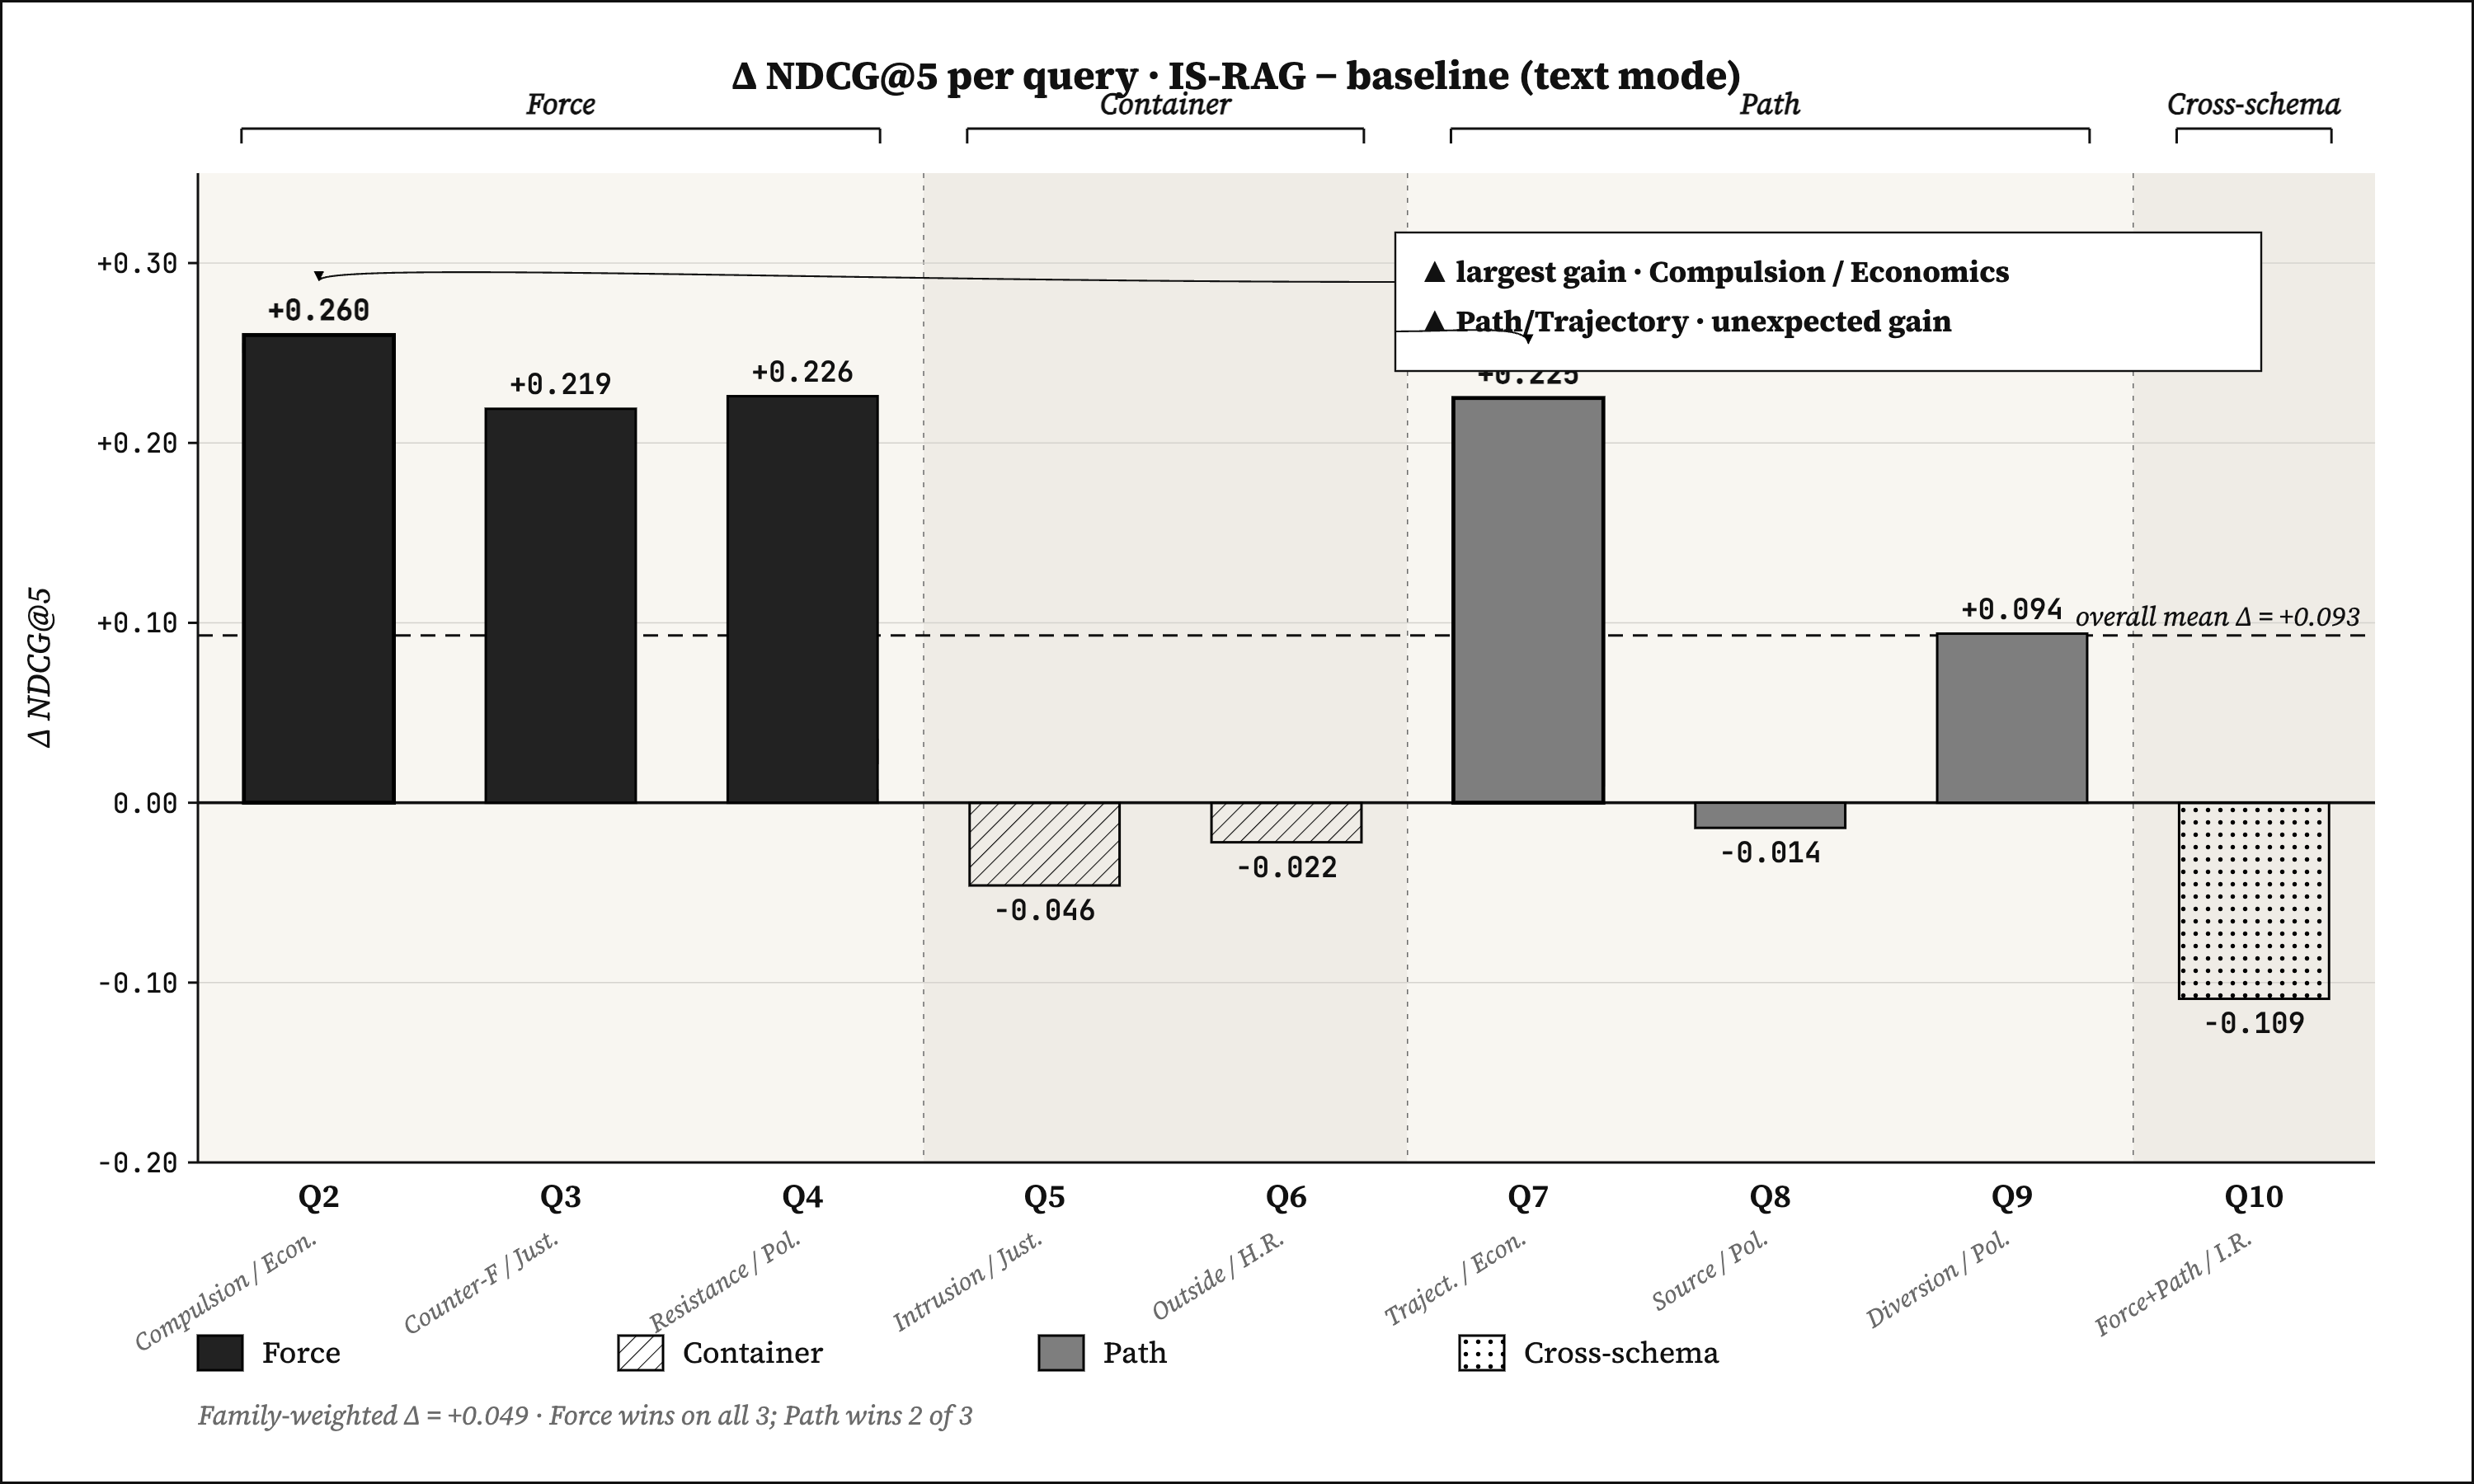
\includegraphics[width=1\textwidth]{images/EN_Results_text_mode.png}
%  \caption{Per-query $\Delta$ NDCG@5 (IS-RAG text mode vs.\ baseline).
%    Queries grouped by schema family; complete values in
%    Table~\ref{tab:perquery}.}
%  \label{fig:results}
%\end{figure}

\subsection{Per-Schema Analysis}

Table~\ref{tab:schema} aggregates text-mode results by schema family
(complete data, all 10~queries).

\begin{table}[h]
\centering
\small
\setlength{\tabcolsep}{4pt}
\begin{tabular}{lccp{4.2cm}}
\toprule
\textbf{Family} & \textbf{$n$} & \textbf{Mean $\Delta$} & \textbf{Individual $\Delta$} \\
\midrule
\textsc{Force}     & 3 & \textbf{+0.267} & +0.390,\ +0.221,\ +0.189 \\
\textsc{Path}      & 3 & +0.085          & +0.036,\ +0.111,\ +0.109 \\
\textsc{Container} & 3 & $-$0.017        & 0.000,\ $-$0.096,\ +0.046 \\
Cross              & 1 & $-$0.094        & $-$0.094 \\
\midrule
\multicolumn{2}{l}{Family-weighted mean} & +0.060 & \\
\bottomrule
\end{tabular}
\caption{NDCG@5 $\Delta$ by schema family (text mode, 10~queries).
  Families ordered by mean~$\Delta$. \textsc{Force} is the strongest
  signal; all three \textsc{Path} queries are now positive.}
\label{tab:schema}
\end{table}

\textsc{Force} shows the strongest and most consistent signal
($\Delta = +0.267$; all three queries positive, peak $+0.390$).
\textsc{Path} is net positive ($+0.085$): all three queries benefit
(Q7~$+0.036$, Q8~$+0.111$, Q9~$+0.109$).
\textsc{Container} shows near-zero mean effect ($-0.017$) across
3~queries: Q1 \textsc{Inside} contributes $\Delta{=}0$
(boost inert for a conventionalised subtype), Q5 \textsc{Intrusion}
$-0.096$, Q6 \textsc{Outside} $+0.046$; all substantially less severe
than in cognitive or hybrid modes (Table~\ref{tab:modes_compare}).
The family-weighted mean ($+0.060$) confirms positive results across
the majority of schema families.

% =================================================================
\section{Discussion}
\label{sec:discussion}

\paragraph{Force benefits most from cognitive boosting.}
All three \textsc{Force} queries show positive~$\Delta$, with
\textsc{Compulsion} ($+0.390$) as the strongest result.
\textsc{Force} schemas tend to use salient, non-conventionalised
metaphorical vocabulary in parliamentary discourse
(\emph{pressiona, bloqueia, choca}), making schema detection and
boosting effective.
This pattern is corpus-specific and should not be generalised without
further validation.

\paragraph{Path is positive across all queries; Container is near-neutral.}
In hybrid mode, \textsc{Path} queries degrade severely
(Q8~$-0.424$, Q7~$-0.007$; Table~\ref{tab:modes_compare}).
In text mode, all three \textsc{Path} queries benefit: Q8~($+0.111$),
Q9~($+0.109$), Q7~($+0.036$); family mean $+0.085$.
The hybrid-mode deficit is therefore an artefact of cognitive-embedding
noise contaminating the base similarity, not an intrinsic property of
trajectory metaphors.
\textsc{Container} shows near-zero mean effect in text mode
($-0.017$ across 3~queries), substantially less severe than in hybrid
or cognitive modes.
Q1 \textsc{Inside} ($\Delta{=}0$) is the key case: even when an
independent annotator finds relevant documents, the cognitive boost
cannot distinguish them — the schema is too conventionalised to carry
a discriminative retrieval signal.

\paragraph{Assertive query formulation is required.}
The Cognitive Parser applies a literality rule: interrogative or
analytical queries (\emph{``Which deputies argue that\ldots''}) are
correctly classified as non-metaphorical, returning empty schema lists
and zeroing the boost.
Queries must be formulated as \emph{assertive metaphorical statements}
to activate the cognitive component.
This is a binding operational constraint for any IS-RAG deployment.

\paragraph{Schema frequency $\neq$ boostability.}
Q1 was designed as \textsc{Container}/\textsc{Inside}, the most
frequent subtype in the corpus (80~occurrences).
The Haiku annotator consistently rated \textsc{Inside} chunks at
score~1 (domain present, schema non-salient), yielding IDCG${=}0$.
The independent Opus annotator finds relevant chunks for Q1 — yet
IS-RAG achieves $\Delta{=}0$ (IS-RAG $=$ baseline $= 0.522$):
cognitive boosting adds nothing even when relevant documents exist.
Spatial containment is so conventionalised in parliamentary discourse
that its schema signal is not discriminative for re-ranking, regardless
of which model judges relevance.
The finding generalises from \emph{annotability} to \emph{boostability}:
the schema is evaluable but carries no useful retrieval signal.
The final query distribution is 3-3-3-1 (10~valid queries).

\paragraph{IS-RAG as a compensatory layer for embedding limitations.}
The embedding experiment (\S\ref{sec:embedding}) positions IS-RAG within
a broader architectural tension: the lexical-cognitive gap the schema
boost bridges is one that SOTA dense models increasingly close
\emph{implicitly} through deeper pre-training on diverse multilingual
corpora.
This makes IS-RAG particularly valuable in deployment scenarios where
large-scale embeddings are impractical --- resource-constrained
environments, on-device retrieval, or regulatory contexts requiring
locally-hosted models --- where explicit schema boosting recovers a
substantial portion of the semantic alignment that stronger embeddings
would otherwise provide natively.
As embedding technology continues to advance, the marginal value of IS-RAG
in text mode is expected to diminish further, motivating future work on
schema-aware retrieval robust to strong base embeddings: domain-specific
fine-tuning of the Cognitive Parser, schema-conditioned re-rankers, or
hard schema constraints rather than soft proportional boosts.
Crucially, hybrid and cognitive degradation remain stable regardless of
embedding quality (\S\ref{sec:embedding}), confirming that the failure
of dual-embedding search is structural rather than model-dependent.

\paragraph{Limitations.}
(1)~The corpus is small and homogeneous (171~chunks, single register,
Portuguese only); results lack statistical significance tests.
(2)~\emph{LLM circularity}: the Cognitive Parser and query parser use
\texttt{claude-haiku-4-5}; the relevance annotator uses
\texttt{claude-opus-4-7} (configurable via \texttt{ANNOTATOR\_MODEL}).
This deliberate model separation breaks the most critical echo loop:
the evaluator is no longer the same model that indexed document
schemas.
Residual risk remains (both are Anthropic/Claude models), and a blind
human audit on a 20\% pool sample will be conducted in future work to
compute Fleiss' Kappa inter-annotator agreement.
(3)~Domain confounding: \textsc{Force} queries cluster in Economics
and Justice; if the schema co-occurs with those domains in the corpus,
gains may reflect domain affinity rather than purely cognitive
structure.
(4)~Boosting weights ($\alpha{=}0.4$, $\beta{=}0.3$) are fixed design
choices, not optimised.
(5)~\emph{Evaluation non-determinism}: the Cognitive Parser introduces
run-to-run variance in IS-RAG scores.
A second independent run yields IS-RAG\,=\,0.7716 ($\Delta=+0.077$,
text mode); the baseline (0.6947) is deterministic and stable.
The positive direction of $\Delta$ is consistent across both runs;
the exact magnitude is not.
Multiple runs with mean\,$\pm$\,std reporting are left for future work.

% =================================================================
\section{Conclusion}
\label{sec:conclusion}

This paper presents IS-RAG as a pioneering pilot study opening a new
line of research at the intersection of cognitive linguistics and
information retrieval.
The core contribution is not a claim of universal superiority, but a
demonstration that image-schema metadata can be encoded, detected, and
leveraged as a proportional re-ranking signal within a standard dense
retrieval pipeline---producing a mean NDCG@5 gain of $+0.091$ in
text-boosting mode (10~queries, Brazilian parliamentary corpus,
independent Opus annotator).
A mode ablation (\S\ref{sec:ablation}) localises the IS-RAG
contribution precisely: the multiplicative boost applied over
text-embedding similarity is effective
($\Delta_\text{text} = +0.091$), while cognitive embeddings used as
search vectors degrade performance
($\Delta_\text{hybrid} = -0.090$; $\Delta_\text{cognitive} = -0.192$).
Crucially, this gain holds under independent annotation
(Table~\ref{tab:annotator}), ruling out LLM echo as its source.
A subsequent experiment with \texttt{BAAI/bge-m3}
(\S\ref{sec:embedding}) reveals that the gain is embedding-dependent:
with a state-of-the-art multilingual model the text-mode $\Delta$
collapses to $\approx 0$, defining a utility frontier for explicit
cognitive boosting.

The asymmetric results across schema families and modes are themselves
findings: they reveal that schema frequency does not predict
boostability, that \textsc{Path} deficits in hybrid mode are artefacts
of noisy cognitive embeddings rather than schema properties, and that
dual-embedding retrieval is not necessary for IS-RAG to work.
IS-RAG establishes the proof of concept and the methodological
scaffolding---cognitive metadata indexing, proportional boosting,
TREC-style schema-stratified evaluation---that future work in
\emph{cognitive IR} can build upon.

Immediate next steps include a schema$\times$domain crossed evaluation
design, investigation of conventionalised schemas in graded-relevance
annotation, cross-register and cross-language validation, and the
Fleiss' Kappa human audit described above.
We invite the IR and cognitive linguistics communities to extend,
challenge, and refine this technique across richer corpora and
retrieval architectures.

% =================================================================
\paragraph*{Code and Data Availability.}
Code, corpus, and annotated ground truth are publicly available at
\url{https://github.com/yanjustino/is-rag}.

% =================================================================
\bibliography{references}

% =================================================================
\appendix
\setcounter{section}{0}
\renewcommand{\thesection}{\Alph{section}}

% =================================================================
\pagebreak
\section{IS-RAG Algorithms}
\label{app:algorithms}

\subsection{Indexing Pipeline}

\begin{algorithm}[h]
\caption{IS-RAG Indexing}\label{alg:index}
\begin{algorithmic}[1]
\Require Corpus $\mathcal{D}$, chunk size $w{=}150$,
         encoder $\mathcal{E}$, LLM parser $\mathcal{P}$
\Ensure  Populated vector store $\mathcal{S}$
\For{each document $d \in \mathcal{D}$}
  \State $C \gets \textsc{SemanticChunk}(d,\,w)$
  \Comment{sentence-boundary split}
  \State $\mathbf{E}_t \gets [\,\mathcal{E}(c) \mid c \in C\,]$
  \Comment{text embeddings, $d$-dim (model-configurable)}
  \State $M \gets [\,\mathcal{P}(c) \mid c \in C\,]$
  \Comment{concurrent LLM calls, 5 workers}
  \For{$i \gets 1$ \textbf{to} $|C|$}
    \State $\mathbf{e}_c \gets \mathcal{E}(\textsc{Serialize}(M_i))$
    \Comment{cognitive embedding}
    \State $\mathcal{S}.\textsc{Insert}(C_i,\,\mathbf{E}_{t,i},\,\mathbf{e}_c,\,M_i)$
  \EndFor
\EndFor
\end{algorithmic}
\end{algorithm}

\subsection{Query-Time Retrieval}

\begin{algorithm}[h]
\caption{IS-RAG Retrieval}\label{alg:retrieve}
\begin{algorithmic}[1]
\Require Query $q$, mode $m \in \{\text{text, cognitive, hybrid}\}$,
         top-$k$, store $\mathcal{S}$, $\alpha{=}0.4$, $\beta{=}0.3$
\Ensure  Ranked list of $k$ chunks
\State $(\Sigma_q, \Delta_q) \gets \mathcal{P}(q)$
\Comment{detected schemas and domains}
\State $\mathbf{e}_{q,t} \gets \mathcal{E}(q)$;\;
       $\mathbf{e}_{q,c} \gets \mathcal{E}(\textsc{Serialize}(\mathcal{P}(q)))$
\For{each chunk $(C_i,\,\mathbf{e}_{t,i},\,\mathbf{e}_{c,i},\,M_i) \in \mathcal{S}$}
  \State $s_t \gets \cos(\mathbf{e}_{q,t},\,\mathbf{e}_{t,i})$;\;
         $s_c \gets \cos(\mathbf{e}_{q,c},\,\mathbf{e}_{c,i})$
  \State $s \gets \begin{cases}
    s_t & \text{if } m = \text{text} \\
    s_c & \text{if } m = \text{cognitive} \\
    (s_t + s_c)/2 & \text{if } m = \text{hybrid}
  \end{cases}$
  \State $n \gets |M_i.\text{details}|$
  \State $\sigma \gets |\{d \in M_i.\text{details} \mid d.\text{schema} \in \Sigma_q\}|
                       \;/\; \max(n,1)$
  \State $\delta \gets |\{d \in M_i.\text{details} \mid d.\text{domain} \in \Delta_q\}|
                       \;/\; \max(n,1)$
  \If{$M_i.\text{schemas} \cap \Sigma_q \neq \emptyset$}
    \State $\hat{s}_i \gets s \cdot (1 + \alpha\,\sigma + \beta\,\delta)$
    \Comment{Eq.~\ref{eq:boosting}}
  \Else
    \State $\hat{s}_i \gets s$
    \Comment{no schema match — no boost}
  \EndIf
\EndFor
\State \Return $\textsc{TopK}(\{\hat{s}_i\},\,k)$
\end{algorithmic}
\end{algorithm}

\end{document}
